\chapter{Implementación y Desarrollo del Sistema}

\begin{quotation}[Novelist]{Ernest Hemingway (1899--1961)}
The good parts of a book may be only something a writer is lucky enough to overhear or it may be the wreck of his whole damn life -- and one is as good as the other.
\end{quotation}

\begin{abstract}
Este capítulo documenta el ciclo de vida del desarrollo de software del proyecto \textit{King and Peasant}, narrando la evolución técnica desde la orquestación inicial de la infraestructura hasta la estabilización funcional del motor asimétrico. El objetivo principal es exponer las decisiones arquitectónicas, algorítmicas y de diseño adoptadas a lo largo de 16 iteraciones iterativas e incrementales. Se detalla la resolución de retos complejos de ingeniería, como la sincronización bidireccional mediante WebSockets, la protección de estados asimétricos a través de DTOs, la gestión de memoria en lógicas de cascada y la automatización del aseguramiento de la calidad. A través de este análisis progresivo, se justifica de forma práctica cómo los requerimientos de fiabilidad, rendimiento y mantenibilidad han sido satisfechos en el producto final.
\end{abstract}

\section{Configuración del Entorno y Arquitectura Base}

\textbf{Flujo de Interacción y Arquitectura} \\
Esta fase establece la orquestación inicial del monorepositorio utilizando espacios de trabajo (\textit{npm workspaces}) para unificar el desarrollo del cliente (\textit{Vite/React}) y el servidor (\textit{Node.js/Express}). La arquitectura se basa en contenedores \textit{Docker}, permitiendo un despliegue aislado de los servicios de infraestructura (\textit{MariaDB} y \textit{Redis}) para garantizar la paridad de entornos locales y facilitar la futura integración continua.

\textbf{Estructura de Directorios} \\
\begin{verbatim}
KingAndPeasant/
|-- docker-compose.yml
|-- packages/
|   |-- client/
|   |   |-- src/
|   |   +-- package.json
|   +-- server/
|       |-- src/
|       +-- package.json
+-- package.json
\end{verbatim}

\textbf{Snippets Estratégicos de Código} \\
\begin{lstlisting}
# docker-compose.yml
version: '3.8'
services: 
  mariadb:
    image: mariadb:10.11
    # ... configuracion interna omitida para resumir el contenido
  redis:
    image: redis:7.0
    # ... configuracion interna omitida
\end{lstlisting}

\subsection{Iteración 1: Configuración de Entornos y Metodología Base}

\textbf{1. Definición de Características} \\
El objetivo primordial de esta primera iteración consistió en establecer los cimientos arquitectónicos e infraestructurales del proyecto \textit{King and Peasant}. Se buscó preparar un entorno de desarrollo robusto que garantizara la paridad entre los entornos de los distintos desarrolladores y sentar las bases de la metodología ágil que guiará el resto del ciclo de vida del software.

\textbf{2. Diseño de la Solución} \\
Para abordar estas características, el diseño se articuló en torno a la orquestación inicial del entorno. A nivel de equipo, se diseñó una estructura de monorepositorio y se redactó el documento de metodología en Markdown para estandarizar el flujo de trabajo (ramas, \textit{commits} y seguimiento de \textit{issues}). A nivel técnico, para satisfacer el requisito de arquitectura (\textbf{RNF-ARQ}), el diseño contempló el uso de \textit{Docker} y \textit{Docker Compose}. La creación de los archivos \texttt{Dockerfile} permitió plantear un despliegue aislado de los entornos de ejecución base (véase la Figura \ref{fig:docker_topology}).

\begin{figure}[H]
\centering
\begin{tikzpicture}[
    scale=0.7, transform shape,
    node distance=2.5cm,
    service/.style={rectangle, draw=ThemeColor1, fill=ThemeColor2, thick, minimum width=3cm, minimum height=1.2cm, align=center, rounded corners},
    infra/.style={cylinder, draw=ThemeColor1, fill=ThemeColor2, thick, minimum width=2cm, minimum height=1.5cm, shape border rotate=90, align=center},
    network/.style={draw=ThemeColor1, dashed, thick, inner sep=0.8cm, rounded corners}
]

    % Services
    \node[service] (client) {Client \\ \small (Vite/React)};
    \node[service, right=of client] (server) {Server \\ \small (Node.js/Express)};
    
    % Infrastructure
    \node[infra, below=1.5cm of server, xshift=-1.5cm] (mariadb) {MariaDB \\ \small (Relational)};
    \node[infra, below=1.5cm of server, xshift=1.5cm] (redis) {Redis \\ \small (In-Memory)};

    % Arrows
    \draw[<->, >=stealth, thick, ThemeColor1] (client) -- node[above, black] {\scriptsize HTTP/WS} (server);
    \draw[->, >=stealth, thick, ThemeColor1] (server) -- node[left, black, xshift=-0.1cm] {\scriptsize SQL} (mariadb);
    \draw[->, >=stealth, thick, ThemeColor1] (server) -- node[right, black, xshift=0.1cm] {\scriptsize Events} (redis);

    % Network box
    \begin{pgfonlayer}{background}
        \node[network, fit=(client) (server) (mariadb) (redis), label={[ThemeColor1]above:Docker Internal Bridge Network}] {};
    \end{pgfonlayer}

\end{tikzpicture}
\caption{Diagrama de topología de contenedores de la infraestructura base, ilustrando la red interna (bridge) entre el servidor, MariaDB y Redis.}
\label{fig:docker_topology}
\end{figure}

\textbf{3. Detalles de Implementación} \\
Para asegurar la cohesión del monorepositorio, se estructuró el proyecto utilizando \textit{npm workspaces}, agrupando el cliente (\textit{Vite/React}) y el servidor (\textit{Node.js}) bajo un único árbol de dependencias. La orquestación se materializó a través de \textit{scripts} centralizados en el \texttt{package.json} raíz, combinando \textit{concurrently} para levantar múltiples entornos de desarrollo en paralelo y \textit{Docker Compose} para inicializar la capa de persistencia. Esto permitió que, mediante un único comando (\texttt{npm run start:local}), el sistema validara la salud de los contenedores y ejecutara las migraciones de base de datos antes de exponer los puertos, eliminando la fricción de configuración inicial.

\textbf{4. Seguimiento, Control y Replanificación} \\
Durante el seguimiento de la orquestación inicial, se detectó una desviación: surgieron conflictos de red que impedían el arranque limpio de los servicios en los contenedores. El control del problema se gestionó unificando la red interna bajo un driver \textit{bridge} personalizado. Tras aplicar esta replanificación técnica, la iteración concluyó satisfactoriamente. La infraestructura base y las políticas del repositorio quedaron operativas, eliminando la fricción inicial y asegurando que el equipo pudiera arrancar con el desarrollo de la capa de datos en el siguiente \textit{sprint} sin arrastrar deuda técnica.

\subsection{Iteración 2: Diseño de Interfaces y Orquestación de Datos}

\textbf{1. Definición de Características} \\
El objetivo establecido para este ciclo, centrado en las responsabilidades individuales de infraestructura y diseño visual, fue sentar las bases de la identidad del proyecto \textit{King and Peasant} mediante la elaboración de \textit{mock-ups} detallados y la orquestación de las bases de datos en el entorno local.

\textbf{2. Diseño de la Solución} \\
El diseño de la solución arrancó con la elaboración de los \textit{mock-ups} completos de las pantallas clave del ecosistema, incluyendo los flujos de autenticación (Login/Registro), las salas de espera (\textit{Lobbies}), el perfil del usuario, el menu principal y el tablero de la partida asimétrica. Esta labor proporcionó una visión estructural clara para el desarrollo en cliente, como se ilustra en la Figura \ref{fig:ui_gameboard}. A nivel de infraestructura, y en cumplimiento del requisito de rendimiento (\textbf{RNF-REN}), el diseño amplió la configuración de \textit{Docker Compose} para incluir el despliegue aislado de los servicios de \textit{MariaDB} y \textit{Redis}.

\begin{figure}[H]
\begin{center}
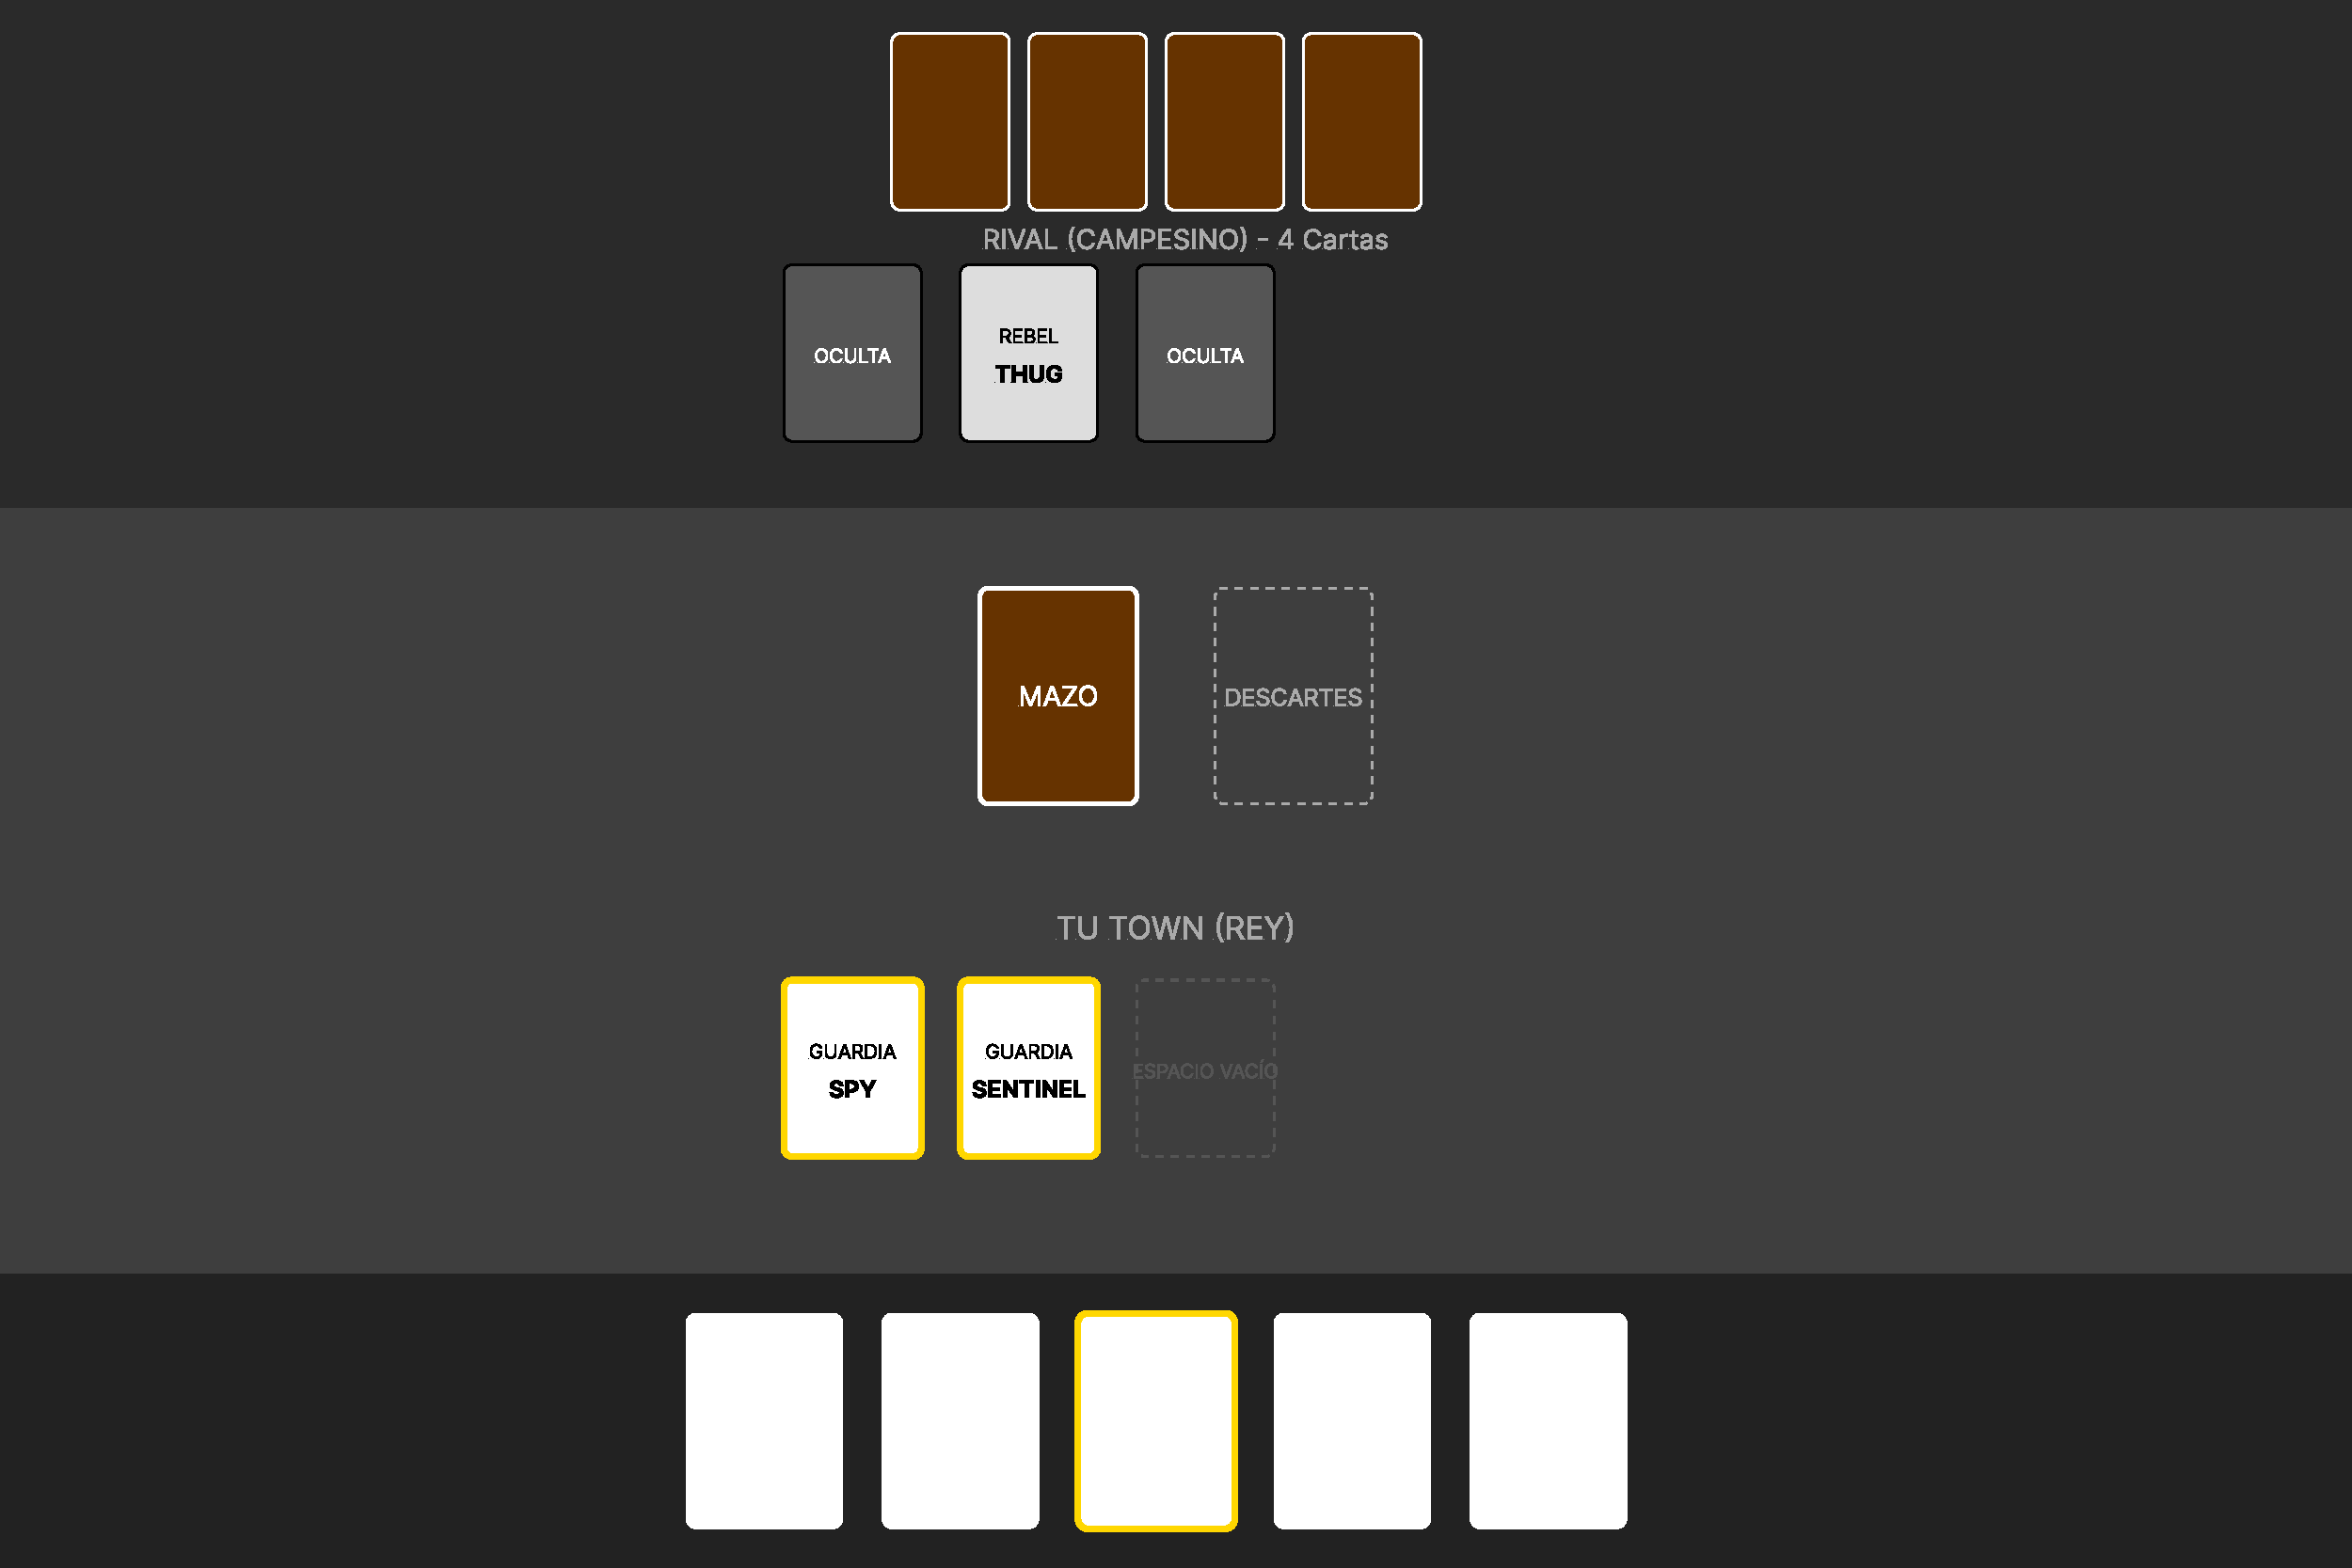
\includegraphics[width=0.9\textwidth]{figures/game_board_ui.pdf}
\caption{Captura de los mock-ups de la interfaz principal: Tablero de juego asimétrico y salas de espera (Lobbies).}
\label{fig:ui_gameboard}
\end{center}
\end{figure}

\textbf{3. Detalles de Implementación} \\
La integración de múltiples motores de bases de datos exigió un desarrollo cauteloso en el archivo \texttt{docker-compose.yml}. Se implementaron volúmenes persistentes (\textit{Volumes}) tanto para \textit{MariaDB} (\texttt{/var/lib/mysql}) como para \textit{Redis} (\texttt{/data}), asegurando que la reinicialización de los contenedores no provocara la pérdida de información crítica. Adicionalmente, se ejecutaron comprobaciones de estado (\textit{healthchecks}) con comandos nativos como \textit{mysqladmin ping} y \textit{redis-cli ping}, garantizando que los servicios de \textit{backend} dependientes (\textit{depends\_on}) no intenten establecer conexiones hasta que los motores estén operativos.

\textbf{4. Seguimiento, Control y Replanificación} \\
Durante el control de la integración del almacenamiento en memoria surgieron bloqueos temporales en la comunicación de los servicios locales. La desviación se resolvió en caliente corrigiendo el mapeo de puertos y exponiendo el 6379 hacia el \textit{localhost} en el \texttt{docker-compose.yml}. Tras esta corrección, las tareas se completaron satisfactoriamente y se integraron en la rama principal, dejando la plataforma preparada para iniciar la estructuración del ORM en la iteración siguiente.

\section{Autenticación y Modelado de Datos}

\textbf{Flujo de Interacción y Arquitectura} \\
El flujo de autenticación implementa el patrón de diseño \textit{Context API} en el \textit{frontend} para inyectar globalmente el estado de sesión del usuario. A nivel de \textit{backend}, se utiliza \textit{Prisma ORM} como intermediario transaccional con la base de datos relacional. Las peticiones a rutas protegidas se validan mediante \textit{middlewares} que decodifican \textit{JSON Web Tokens (JWT)}, logrando una arquitectura de seguridad robusta y desacoplada.

\textbf{Estructura de Directorios} \\
\begin{verbatim}
packages/
|-- client/src/
|   +-- context/
|       +-- AuthContext.ts
+-- server/
    |-- prisma/
    |   +-- schema.prisma
    +-- src/controllers/
        +-- UserController.js
\end{verbatim}

\textbf{Snippets Estratégicos de Código} \\
\begin{lstlisting}[language=Java]
// packages/client/src/context/AuthContext.ts
interface AuthContextType {
  user: User | null;
  isLogin: boolean;
  login: (userData: User) => void;
  // ... logica interna omitida para resumir el contenido
  socket: Socket | null;
}
export const AuthContext = createContext<AuthContextType | undefined>(undefined);
\end{lstlisting}

\begin{lstlisting}[language=Java]
// packages/server/prisma/schema.prisma
model User {
  idUser   Int      @id @default(autoincrement())
  name     String   @unique
  email    String   @unique
  password String
  // ... resto de campos relacionales omitidos
}
\end{lstlisting}

\subsection{Iteración 3: Modelado Estructural y Flujo de Negocio}

\textbf{1. Definición de Características} \\
El objetivo principal asignado para esta iteración se centró en la conceptualización teórica del dominio de datos, así como en el modelado formal del flujo que gobernaría la asimetría de las partidas.

\textbf{2. Diseño de la Solución} \\
El diseño de esta etapa se articuló en torno a la arquitectura de la información. Se elaboró el modelo Entidad-Relación y el diagrama UML correspondiente a la base de datos relacional. De forma paralela, el equipo diseñó los estados de la partida, los turnos intercalados y las mecánicas asimétricas plasmándolas en diagramas de flujo operativos.

\textbf{3. Detalles de Implementación} \\
El diseño estructural requirió abstraer la asimetría del juego a un modelo de datos cohesivo. El esquema relacional implementó entidades independientes para \texttt{User}, \texttt{Friendship}, \texttt{Lobby} y \texttt{Game}. La complejidad se centró en la entidad \texttt{Card}, la cual fue codificada para contener tanto los atributos del bando del Rey (\texttt{nameKing}, \texttt{typeKing}) como los del Campesino (\texttt{namePeasant}, \texttt{typePeasant}) en un mismo registro. Esto facilitó enormemente la futura gestión del mazo único compartido. Las relaciones múltiples reflexivas en la entidad \texttt{User} (como \texttt{gamesAsPlayer1} o \texttt{friendshipsSent}) se implementaron para permitir consultas eficientes de historiales y marcadores.

\textbf{4. Seguimiento, Control y Replanificación} \\
El seguimiento de este \textit{sprint} arrojó resultados óptimos. Los objetivos de modelado de datos y flujos lógicos se alcanzaron con éxito, sin registrarse desviaciones temporales ni bloqueos técnicos que obligaran a replanificar. El diseño quedó certificado y listo para ser trasladado al ORM en la siguiente iteración.

\subsection{Iteración 4: Implementación del Modelo Estructural para los usuarios}

\textbf{1. Definición de Características} \\
El objetivo principal para esta iteración se basó en la implementación técnica del modelo de datos diseñado previamente en la base de datos relacional, haciendo uso del modelo Entidad-Relación y el diagrama UML correspondiente.

\textbf{2. Diseño de la Solución} \\
En cumplimiento con el requisito de arquitectura (\textbf{RNF-ARQ}), el diseño de la solución dictaminó que este modelo conceptual se trasladara al entorno de desarrollo utilizando \textit{Prisma ORM}. Se diseñó una estrategia basada en migraciones secuenciales sobre el despliegue aislado de \textit{MariaDB}, garantizando que el esquema de la base de datos estuviera en sincronía con el contenedor de Docker.

\textbf{3. Detalles de Implementación} \\
La transición del modelo a la infraestructura real se codificó definiendo el esquema en \texttt{schema.prisma}. Esta implementación generó automáticamente un cliente tipado para \textit{Node.js}, proporcionando autocompletado y seguridad de tipos en la capa de controladores. La ejecución de las migraciones (\texttt{prisma migrate}) actuó como un sistema de control de versiones sobre \textit{MariaDB}, garantizando que cualquier cambio en la estructura de tablas o índices (como \texttt{@@unique([idSender, idReceiver])} en las amistades) se aplicase de forma atómica.

\textbf{4. Seguimiento, Control y Replanificación} \\
Durante el control de calidad de la iteración no se reportaron fallos en las transacciones de las migraciones. El modelo de datos se materializó en los contenedores locales sin desviaciones, cerrando la iteración en el tiempo estipulado y permitiendo continuar con la capa de seguridad.

\subsection{Iteración 5: Gestión de Identidad, Seguridad y Perfiles}

\textbf{1. Definición de Características} \\
El objetivo primordial de este ciclo consistió en implementar de forma integral la capa de gestión de usuarios del ecosistema. Esto abarcó tanto la seguridad del acceso (registro y autenticación de credenciales) como la administración de la identidad digital del jugador, proporcionando una zona privada para la edición de datos personales y la visualización de estadísticas de juego.

\textbf{2. Diseño de la Solución} \\
El diseño de la solución abordó la construcción de las vistas operativas de \textit{Login}, \textit{Register} y el panel de \textit{Profile}. Dando cumplimiento al requisito de seguridad (\textbf{RNF-SEG}), el diseño de la lógica del servidor se basó en la emisión y validación de \textit{JSON Web Tokens} (JWT), asegurando el encriptado unidireccional de contraseñas. Para el cliente, se diseñaron formularios reactivos integrados con un contexto global de autenticación para gobernar las rutas privadas.

\textbf{3. Detalles de Implementación} \\
El núcleo de la seguridad se implementó codificando la ofuscación de contraseñas con \textit{bcrypt} durante el registro. En la autenticación exitosa, el \textit{backend} firma un JWT empaquetando el identificador del usuario. El \textit{frontend} inyecta este \textit{token} como cabecera en cada petición HTTP protegida. Un \textit{middleware} programado en \textit{Node.js} intercepta estas peticiones, verificando la validez criptográfica de la firma antes de permitir el acceso a controladores restringidos mediante \textit{Prisma ORM}.

\textbf{4. Seguimiento, Control y Replanificación} \\
El seguimiento de la integración detectó desviaciones severas en el cliente y el servidor. En el \textit{frontend}, surgieron dificultades con la persistencia del estado de sesión; se replanificó implementando un \textit{AuthContext} en \textit{React}. En el \textit{backend}, el diseño inicial de los controladores mezclaba validaciones con persistencia. Se aplicó una refactorización correctiva orientada a la separación de responsabilidades. Tras estas acciones de control, la iteración concluyó satisfactoriamente unificando los flujos de acceso.

\section{Interacciones Sociales y Comunicación Bidireccional}

\textbf{Flujo de Interacción y Arquitectura} \\
Para resolver la latencia en la interacción social (sistema de amigos y futuras mecánicas de partida), se sustituye el modelo tradicional de \textit{HTTP Polling} por una conexión persistente bidireccional basada en el protocolo \textit{WebSockets} utilizando \textit{Socket.io}. La arquitectura se modela mediante un \textit{Socket Manager} en el servidor, implementado bajo un patrón \textit{Singleton}, que gestiona la emisión de eventos (\textit{Broadcast}) a salas específicas y propaga notificaciones en tiempo real a los clientes conectados.

\textbf{Estructura de Directorios} \\
\begin{verbatim}
packages/server/src/
|-- controllers/
|   +-- FriendshipController.js
+-- sockets/
    +-- LobbySocket.js
\end{verbatim}

\textbf{Snippets Estratégicos de Código} \\
\begin{lstlisting}[language=Java]
// packages/server/src/sockets/LobbySocket.js
const registerLobbyHandlers = (io, socket) => {
  // ... configuracion interna omitida para resumir el contenido
  socket.on("createLobby", async (lobbyName, isPrivate) => {
      // ... logica de emision de eventos omitida
  });
}
\end{lstlisting}

\subsection{Iteración 6: Interacciones Sociales y Comunicación en Tiempo Real}

\textbf{1. Definición de Características} \\
El objetivo establecido para este ciclo fue implementar el componente social del ecosistema, diseñando un sistema de amistades entre usuarios e introduciendo la base técnica para la comunicación bidireccional necesaria en la futura partida.

\textbf{2. Diseño de la Solución} \\
El diseño se dividió en dos frentes. Por un lado, se planificaron los \textit{endpoints} y el modelo de entidad relacional para enviar, aceptar y rechazar amistades, junto con su vista (\textit{Dashboard}). Por otro lado, en cumplimiento del requisito de rendimiento (\textbf{RNF-REN}), se diseñó la sustitución del protocolo HTTP tradicional por \textit{WebSockets} (\textit{Socket.io}) en el servidor. La justificación arquitectónica de esta decisión se detalla en la Tabla \ref{tab:ws_analisis}.

\begin{table}[H]
\centering
\begin{coolTable}{p{4cm}p{\textwidth-4.5cm}}{2}
{Análisis de valor: Comunicación por WebSockets}
\textbf{Propuesta}&Sustitución del paradigma HTTP tradicional (REST) por un canal persistente bidireccional basado en Socket.io.\\
\midrule
\textbf{Valor}&Garantiza latencia casi nula para la sincronización de las mecánicas de partida y notificaciones de amistad.\\
\textbf{Coste}&Aumenta la complejidad de la infraestructura al requerir un \textit{Socket Manager} y mayor consumo de memoria por conexiones abiertas.\\
\textbf{Opciones}&\textit{HTTP Long Polling} o \textit{Server-Sent Events (SSE)}, descartadas por sobrecarga de red y limitación unidireccional respectivamente.\\
\textbf{Riesgos}&Riesgo crítico de fugas de memoria (\textit{memory leaks}) ante desconexiones no gestionadas de los clientes.\\
\textbf{Deuda técnica}&Obliga a implementar lógicas manuales de reconexión y ciclos de limpieza (\textit{cleanup}) en el frontend (React).\\
\end{coolTable}
\caption{Análisis de valor aportado sobre la arquitectura de comunicación mediante WebSockets. \label{tab:ws_analisis}}
\end{table}

\textbf{3. Detalles de Implementación} \\
El principal desafío de implementación consistió en mantener una única fuente de verdad sincronizada. El algoritmo desarrollado operó estableciendo un mapa en memoria en el servidor que vincula el \texttt{userId} con su \texttt{socket.id}. Tras completarse una transacción en \textit{MariaDB} (ej. aceptar una solicitud), el controlador invoca al gestor de \textit{Sockets}. Éste emite un evento tipado (\textit{Broadcast} dirigido) enviando el nuevo estado del \textit{Dashboard}, forzando a la vista \textit{React} a re-renderizarse de forma reactiva sin necesidad de sondeo.

\textbf{4. Seguimiento, Control y Replanificación} \\
Durante el control de calidad de la comunicación, se detectaron dificultades persistentes para establecer una conexión estable (fugas de memoria por múltiples instancias por usuario). La desviación se mitigó replanificando la lógica del cliente e implementando retornos de limpieza (\textit{cleanup}) en los \textit{hooks} de \textit{React} para forzar la desconexión explícita. El ciclo concluyó exitosamente, dejando el motor de comunicación listo para iniciar el flujo principal de la partida.

\section{Arquitectura del Motor de Juego Asimétrico}

\textbf{Flujo de Interacción y Arquitectura} \\
El núcleo funcional del proyecto delega el estado asimétrico de las partidas a un servicio especializado (\textit{Game Service}) que interactúa con la base de datos en memoria \textit{Redis} para minimizar la latencia. El intercambio de información entre servidor y cliente se rige por Objetos de Transferencia de Datos (\textit{DTO}), filtrando atributos confidenciales antes de emitir actualizaciones por \textit{WebSockets}. Las mecánicas asíncronas, como \textit{Pending Actions}, pausan y retoman el hilo de ejecución mediante identificadores únicos.

\textbf{Estructura de Directorios} \\
\begin{verbatim}
packages/
|-- client/src/pages/game/
|   +-- components/
|       +-- GameService.tsx
+-- server/src/
    |-- services/
    |   +-- GameService.js
    +-- controllers/
        +-- GameController.js
\end{verbatim}

\textbf{Snippets Estratégicos de Código} \\
\begin{lstlisting}[language=Java]
// packages/server/src/services/GameService.js
const playActionCard = async (gameId, targetData, playedCard, userRol, gameState) => {
  // ... logica interna de validacion y estado en Redis omitida
}
  
const resolvePendingAction = async (gameId, userId, targetData) => {
  // ... logica de resolucion transaccional omitida
}
\end{lstlisting}

\subsection{Iteración 7: Documentación, Planificación y QA}

\textbf{1. Definición de Características} \\
El objetivo inicial de la iteración consistía en comenzar el desarrollo técnico del motor de juego y el chat en partida. Sin embargo, ante el rápido crecimiento del proyecto, el equipo decidió estratégicamente pivotar los esfuerzos hacia una auditoría profunda del código existente, evaluando las funcionalidades implementadas hasta la fecha para identificar y catalogar la deuda técnica acumulada.

\textbf{2. Diseño de la Solución} \\
Al paralizar el desarrollo de nuevas características, el diseño se centró en elaborar un plan de auditoría. Dando cumplimiento al requisito de mantenibilidad (\textbf{RNF-MAN}), se diseñó un protocolo de revisión de los flujos de datos entre cliente y servidor, con el fin de detectar problemas de escalabilidad visual y riesgos de sobreexposición de datos sensibles en red que podrían comprometer la arquitectura asimétrica futura.

\textbf{3. Detalles de Implementación} \\
Durante este periodo, la ejecución técnica se limitó a tareas de inspección de código estático y análisis de tráfico de red. Se identificaron vulnerabilidades estructurales en la serialización de datos enviados por \textit{WebSockets} y un alto nivel de acoplamiento en los componentes de \textit{React}, documentando exhaustivamente cada hallazgo en el sistema de control de versiones (\textit{Issues}).

\textbf{4. Seguimiento, Control y Replanificación} \\
El control de este \textit{sprint} representó un punto de inflexión crítico. La auditoría demostró que era inasumible continuar el desarrollo sin sanear el núcleo del sistema. Como medida de replanificación, el equipo modificó la pila de producto (\textit{Product Backlog}), arrastrando el desarrollo del chat y priorizando una refactorización masiva para el siguiente ciclo. Se asumió el riesgo consciente de que ciertas características menores quedarían fuera del alcance del proyecto a cambio de garantizar la integridad de la arquitectura central.

\subsection{Iteración 8: Refactorización y Estado Inicial de Partida}

\textbf{1. Definición de Características} \\
El objetivo de este \textit{sprint} fue ejecutar la reestructuración profunda dictaminada en la auditoría previa para mejorar la legibilidad del código. Adicionalmente, se fijó el hito de preparar la base de datos para la configuración del estado inicial de la partida (cartas y mazos).

\textbf{2. Diseño de la Solución} \\
Para cumplir el requisito de mantenibilidad (\textbf{RNF-MAN}), el diseño de la refactorización dictó unificar la nomenclatura y extraer componentes reutilizables en \textit{React}. A nivel de arquitectura (\textbf{RNF-ARQ}), se diseñó el uso del patrón \textit{Data Transfer Object} (DTO) para aislar la \textit{lógica de negocio} de los datos emitidos por red, asegurando la naturaleza "ciega" del juego asimétrico. Además, se planificaron los \textit{seeders} de la base de datos.

\textbf{3. Detalles de Implementación} \\
La vulnerabilidad estructural descubierta se mitigó codificando funciones adaptadoras (\textit{mappers}) puras. Estas rutinas reciben el estado absoluto del juego desde \textit{Redis} y construyen un nuevo objeto purgado para el \textit{socket} receptor. De este modo, propiedades sensibles como la mano del rival se procesan y se envían únicamente como conteos de longitud (números enteros), garantizando que el cliente no pueda inspeccionar el tráfico para obtener ventajas ilícitas.

\textbf{4. Seguimiento, Control y Replanificación} \\
Durante la validación de la refactorización, el seguimiento reveló brechas en el filtrado de datos (ej. \textit{Rival town dto}), que seguían exponiendo información privada. El control de calidad forzó a replanificar la serialización JSON, introduciendo validadores estrictos en los \textit{mappers}. Tras superar este reto, la base de código quedó notablemente robusta y lista para iniciar el sistema funcional de cartas.

\subsection{Iteración 9: Desarrollo del Motor de Juego y Cartas de Acción}

\textbf{1. Definición de Características} \\
El objetivo establecido consistió en dotar de vida al motor de \textit{King and Peasant}, centrándose en la implementación funcional de las cartas de acción y el complejo sistema de acciones pendientes (\textit{Pending Actions}) para manejar la interactividad asimétrica de la partida.

\textbf{2. Diseño de la Solución} \\
El diseño de la solución abordó la creación de los servicios (\textit{Game Service}) y controladores encargados de procesar el uso de cartas, validando la capacidad asimétrica del tablero (\textbf{RN-02}) y automatizando el cierre de turno (\textbf{RN-04}). En el cliente, se diseñaron las interfaces dinámicas para explorar la pila de descartes y el diccionario visual de acciones.

\textbf{3. Detalles de Implementación} \\
El problema computacional residía en congelar el estado del motor de forma segura delegando el contexto a \textit{Redis}. El sistema de cola de acciones (\textit{Pending Actions}) se implementó generando un objeto \texttt{pendingAction} que bloquea algorítmicamente el turno global. Cuando el cliente envía la resolución, un despachador dinámico invoca la función específica requerida, aplica las mutaciones, purga la acción y reactiva el turno, tal y como se formaliza en la Tabla \ref{tab:pending_actions}.

\begin{table}[htbp]
\centering
\begin{asigResponsabilidad}{game-001}{Resolución Pending Actions}
{[Object] resolvePendingAction (gameId:String, userId:Int, targetData:Object)}
\pasoPseudo{Recuperar el estado actual (\texttt{gameState}) almacenado en Redis mediante el \texttt{gameId}.}
\pasoPseudo{Validar que el \texttt{userId} de la petición coincide con el jugador que tiene el foco activo en el objeto \texttt{pendingAction}.}
\pasoPseudo{Invocar al despachador de cartas para aplicar el efecto mecánico sobre el \texttt{targetData}.}
\pasoPseudo{Si la resolución es exitosa, aplicar las mutaciones y purgar el objeto \texttt{pendingAction} del estado general.}
\pasoPseudo{Transicionar el foco y guardar el nuevo estado atómico en Redis.}
\end{asigResponsabilidad}
\caption{Descripción algorítmica de la resolución de acciones asíncronas en el servidor. \label{tab:pending_actions}}
\end{table}

\textbf{4. Seguimiento, Control y Replanificación} \\
El control de la implementación reportó complicaciones severas al sincronizar las mecánicas asíncronas del servidor con la vista. Al aplicar reglas estrictas (\textbf{RN-03}), se originaron bloqueos en la selección de cartas. La desviación obligó a replanificar el control de flujo en \textit{React}, aislando la resolución de las promesas del ciclo de vida de los modales. Solventado esto, el hito crítico se alcanzó, permitiendo la interactividad en mesa.

\subsection{Iteración 10: Condiciones de Victoria y Resolución de Partida}

\textbf{1. Definición de Características} \\
El objetivo fue definir la finalización algorítmica de las partidas, estableciendo las condiciones de victoria asimétricas de cada facción (Guardias vs. Asesino/Revueltas) y puliendo mecánicas clave de final de juego.

\textbf{2. Diseño de la Solución} \\
Para garantizar la atomicidad de victoria (\textbf{RN-05}), el diseño de la lógica de negocio exigió que el motor comprobara de forma asíncrona la victoria tras cada movimiento. Se ideó una orquestación transaccional para asegurar que, al detectar un ganador, \textit{MariaDB} reflejara el cambio de estado, la caché en memoria se bloqueara y el cliente renderizara modales dinámicos de cierre.

\textbf{3. Detalles de Implementación} \\
La complejidad se abordó programando un interceptor central de validación. Tras cualquier mutación en \textit{Redis}, el algoritmo evalúa en paralelo las condiciones absolutas del Campesino frente a las del Rey. Si una aserción retorna un estado ganador válido, el motor consolida el estado en \textit{MariaDB} dentro de una misma transacción de \textit{Prisma}, y envía un código de interrupción por \textit{WebSockets} que destruye el hilo de memoria para evitar condiciones de carrera.

\textbf{4. Seguimiento, Control y Replanificación} \\
Durante las pruebas de transición final, el equipo de control detectó errores de concurrencia que desencadenaban un Error 500 en el servidor al intentar actualizar el estado y destruir el hilo simultáneamente. La corrección requirió replanificar el \texttt{GameController}, encapsulando las sentencias en un bloque transaccional \textit{try/catch} con \textit{await}. Tras la corrección, el motor logró determinar a un ganador de forma robusta.

\section{Aseguramiento de Calidad y Pulido Final}

\textbf{Flujo de Interacción y Arquitectura} \\
La estrategia de validación final adopta un enfoque orientado al aseguramiento de la calidad mediante pruebas de integración automáticas. A nivel de infraestructura, se utiliza el motor \textit{Jest} para instanciar el \textit{Game Service} y los servicios de usuarios junto con bases de datos aisladas en memoria. Esto permite simular con precisión el flujo asimétrico de la partida, certificando la invariabilidad algorítmica de las condiciones de victoria y mitigando la aparición de regresiones indeseadas tras refactorizaciones de última hora.

\textbf{Estructura de Directorios} \\
\begin{verbatim}
packages/
+-- server/
    +-- tests/
        |-- gameService.test.mjs
        |-- userRoutes.test.mjs
        +-- userService.test.mjs
\end{verbatim}

\textbf{Snippets Estratégicos de Código} \\
\begin{lstlisting}[language=Java]
// packages/server/tests/gameService.test.mjs
describe('gameService', () => {
  test('startGame inicializa la partida correctamente con las reglas de King and Peasant', async () => {
     // ... logica interna de aserciones y simulacion omitida
  });
});
\end{lstlisting}

\subsection{Iteración 11: Interfaces Asíncronas y Modales de Cartas de Acción}

\textbf{1. Definición de Características} \\
El objetivo fundamental consistió en desarrollar la capa visual e interactiva del núcleo del juego, implementando el \textit{frontend} de las Cartas de Acción y el complejo sistema de Acciones Pendientes (\textit{Pending Actions}) para permitir a los jugadores reaccionar a eventos asimétricos.

\textbf{2. Diseño de la Solución} \\
Para cumplir el requisito de rendimiento (\textbf{RNF-REN}), el diseño planteó traducir la lógica del servidor a una experiencia reactiva. Se proyectó un diccionario visual unificado (\texttt{pendingActionsUI.tsx}) capaz de instanciar modales específicos (como el ataque \textit{Strike} del Rey) congelando la interfaz general sin perder el contexto visual del tablero.

\textbf{3. Detalles de Implementación} \\
El diccionario dinámico se implementó mapeando las claves de acción del servidor con sus respectivos componentes en \textit{React}. Cuando \textit{Socket.io} notifica un estado con \texttt{pendingAction}, el cliente evalúa si el foco recae en el jugador local. En caso afirmativo, se invoca el componente del diccionario forzando la decisión del usuario y bloqueando algorítmicamente el resto de interacciones (\textit{force play}) hasta que el controlador del servidor resuelva la promesa asíncrona.

\textbf{4. Seguimiento, Control y Replanificación} \\
Durante el acoplamiento del diccionario, el control de la interfaz detectó desajustes visuales (\textit{frontend bugs}) al intentar interactuar con el mazo general mientras un modal estaba activo. Este defecto forzó una replanificación en la jerarquía de dependencias de \textit{React}, reescribiendo los \textit{hooks} para forzar el paso de turno únicamente cuando se confirmaba el retorno HTTP/WS 200 desde el servidor, estabilizando así el flujo.

\subsection{Iteración 12: Consolidación Funcional del Motor de Juego y Lógica de Cartas}

\textbf{1. Definición de Características} \\
El propósito consistió en consolidar el abanico completo de funcionalidades mecánicas de las cartas de ambos bandos, asegurando que las acciones asimétricas complejas (como tácticas de guardias o emboscadas) se resolvieran de forma íntegra.

\textbf{2. Diseño de la Solución} \\
Dando cumplimiento al requisito de funcionalidad (\textbf{RNF-FUN}), el diseño algorítmico orquestó rutinas para alterar el estado de las entidades, calcular daños, escudos y penalizaciones de forma atómica. En el \textit{frontend}, el diseño contempló la incorporación de modales dinámicos para visualizar mazos durante la partida.

\textbf{3. Detalles de Implementación} \\
La programación de acciones múltiples (ej. una carta que permite mirar la mano rival y descartar una carta) se implementó bifurcando el \textit{GameService}. El servidor valida la orden y crea el \texttt{pendingAction}, inyectando al cliente los datos temporales. Una vez tomada la decisión, la resolución final unifica las propiedades alteradas y reanuda el turno general purgando la caché diferida de \textit{Redis}, garantizando una ejecución inmutable.

\textbf{4. Seguimiento, Control y Replanificación} \\
El control de calidad evidenció fricciones temporales al enlazar el diccionario visual con resoluciones múltiples encadenadas. Las respuestas de validación fallaban. Como medida correctiva, se replanificó la arquitectura de respuestas del \textit{GameService} para homogeneizar los formatos de transferencia (DTO) en cada paso de validación intermedia, dejando el sistema de cartas prácticamente completado.

\subsection{Iteración 13: Interfaces de Infiltración y Estabilización del Bucle de Partida}

\textbf{1. Definición de Características} \\
El objetivo fue completar la capa de presentación de la mecánica especial de Infiltración y garantizar la robustez algorítmica del bucle de partida (transiciones entre Eras y validaciones deterministas).

\textbf{2. Diseño de la Solución} \\
Para asegurar la fiabilidad (\textbf{RNF-FIA}), el diseño requirió crear un componente reactivo (\texttt{InfiltrateModal.tsx}) acoplado al diccionario de acciones, dotando al jugador de una vista controlada para examinar la mano rival. Paralelamente, se diseñó la estabilización de los scripts de entorno local (\texttt{npm run start:local}) y del bloque de aserciones de victoria (\textit{Win Condition}) en el servidor.

\textbf{3. Detalles de Implementación} \\
El componente \textit{React} fue programado para capturar el DTO efímero y congelar el entorno de la partida. Su estado visual se coordinó estrictamente con la respuesta asíncrona del servidor, asegurando que los modales se desmontaran limpiamente y reanudaran el cauce natural de turnos tras la alteración exitosa en la base de datos de memoria.

\textbf{4. Seguimiento, Control y Replanificación} \\
Las pruebas del bucle final de juego levantaron una alerta crítica: la invocación a \texttt{setupNewEra} corrompía la asignación de cartas en memoria al cambiar de fase. La desviación exigió replanificar los ciclos del \textit{GameService}, reescribiendo desde cero las funciones de reasignación y limpieza de manos para asegurar que la nueva Era comenzara de forma determinista.

\subsection{Iteración 14: Pulido de Reglas, Corrección de Errores y Refactorización Estructural}

\textbf{1. Definición de Características} \\
El propósito central consistió en el pulido exhaustivo de las reglas del juego (Guardias, Revueltas, Asesino) y el arreglo de errores arrastrados. Además, se fijó el objetivo de optimizar la mantenibilidad del código (\textbf{RNF-MAN}) del \textit{frontend}.

\textbf{2. Diseño de la Solución} \\
El diseño para refactorizar la excesiva complejidad del componente principal (\texttt{Game.tsx}) se fundamentó en tres pilares: extraer la lógica transaccional a \textit{Custom Hooks}, descomponer el árbol JSX en componentes atómicos (\texttt{PlayerArea.tsx}, \texttt{RivalArea.tsx}), y encapsular todas las interfaces de interrupción (\textit{Modals}) para mitigar re-renderizados.

\textbf{3. Detalles de Implementación} \\
A nivel de reglas, se programaron las correcciones matemáticas en los cálculos de letalidad. En la capa de \textit{frontend}, la refactorización se materializó separando el estado global de suscripciones a \textit{WebSockets} hacia \texttt{useGameActions.ts} y \texttt{useGameData.ts}. Adicionalmente, se codificó un nuevo sistema de notificaciones (\texttt{ErrorToast.tsx}) para interceptar y renderizar los errores enviados por el servidor.

\textbf{4. Seguimiento, Control y Replanificación} \\
Durante las pruebas de estrés de este ciclo, el control de errores cazó un fallo 500 no controlado en el cierre de sesiones. Este defecto crítico se solucionó encapsulando el cierre de la partida en una gestión robusta de excepciones. Esta acción correctiva dejó una base limpia y altamente estable.

\subsection{Iteración 15: Sistema de Notificaciones Globales y Alertas de Partida}

\textbf{1. Definición de Características} \\
El objetivo técnico fue interceptar eventos asíncronos críticos transversales (como la finalización oficial de una partida o el abandono de salas de espera) y comunicarlos de forma inmediata mediante modales reactivos, mejorando el \textit{feedback} global.

\textbf{2. Diseño de la Solución} \\
Dando cumplimiento al requisito de usabilidad, el diseño propuso la creación del componente \texttt{AnnouncementModal.tsx}. La arquitectura planificó inyectarlo en la capa superior de la aplicación para interceptar los estados tanto en \texttt{Game.tsx} como en \texttt{LobbyRoom.tsx}, manteniéndolo oculto por defecto.

\textbf{3. Detalles de Implementación} \\
La integración se programó ampliando el estado global en los \textit{hooks} personalizados para escuchar de forma activa las interrupciones de \textit{Socket.io}. Al emitirse una notificación de victoria o abandono, el motor reactivo de estado dispara el modal, bloqueando la interfaz subyacente para forzar la navegación del usuario hacia una zona segura (como el menú principal) e invalidando las interacciones residuales.

\textbf{4. Seguimiento, Control y Replanificación} \\
El seguimiento de la implementación reportó conflictos de renderizado: el modal retenía información obsoleta tras salidas abruptas de los \textit{Lobbies}. La solución requirió replanificar el ciclo de vida de desmontaje en \textit{React}, añadiendo lógicas estrictas para purgar las suscripciones a \textit{WebSockets} antes de destruir la vista. Tras esto, las notificaciones funcionaron de forma impecable.

\subsection{Iteración 16: Automatización de Pruebas y Validación Integral del Sistema}

\textbf{1. Definición de Características} \\
El objetivo de este \textit{sprint} se centró en asegurar la calidad del software mediante la automatización de pruebas, blindando la \textit{lógica de negocio} del motor asimétrico y las interfaces, garantizando así la fiabilidad (\textbf{RNF-FIA}) del producto.

\textbf{2. Diseño de la Solución} \\
Se diseñó una \textit{suite} de pruebas utilizando el motor \textit{Jest}. La arquitectura de validación simuló servicios de usuarios y el \textit{Game Service} operando contra bases de datos aisladas en memoria. En \textit{frontend}, el diseño abarcó pruebas de componentes mediante DOM virtual para verificar los flujos de inicio de sesión y gestión de perfil.

\textbf{3. Detalles de Implementación} \\
Las pruebas automatizadas lograron exponer fragilidades en lógicas de cascada (como \textit{Revolt}). La refactorización exigió aislar las mutaciones de poder en buffers temporales. Se codificó una resolución en cascada estricta, asegurando que los eventos masivos no sobreescribieran referencias de memoria. Esta aproximación garantizó que, si el sistema asíncrono detectaba un fallo, la operación atómica abortara preservando la partida intacta.

\textbf{4. Seguimiento, Control y Replanificación} \\
Durante el monitoreo de la \textit{suite}, el sistema reportó discrepancias graves en \textit{Redis}: mecánicas letales (\textit{Strike}) no aplicaban el daño correctamente. El equipo pausó la creación de nuevos \textit{tests} y replanificó el esfuerzo para reescribir parte de la lógica en los \textit{pendingActions} defectuosos. Tras iterar sobre el código, la tasa de éxito de las pruebas alcanzó el 100\%, validando la estabilidad definitiva del software.

\subsection{Iteración 17: Redacción Técnica y Consolidación Documental}

\textbf{1. Definición de Características} \\
El objetivo primordial de este ciclo final consistió en intensificar la producción de la memoria técnica del proyecto, liberando ancho de banda y presión administrativa para afrontar la entrega definitiva.

\textbf{2. Diseño de la Solución} \\
La solución metodológica planteó detener el desarrollo de nuevas características y establecer un flujo de redacción concurrente. El diseño documental exigió justificar las decisiones arquitectónicas previas y estructurar todos los artefactos visuales (diagramas UML, tablas de análisis) generados a lo largo de los 16 \textit{sprints} anteriores.

\textbf{3. Detalles de Implementación} \\
La ejecución se centró en el trabajo sobre el proyecto \textit{LaTeX}. Se unificó el estilo narrativo del equipo y se resolvieron errores tipográficos y de compilación (\textit{Overfull hboxes}). La redacción se abordó con revisiones cruzadas constantes frente al repositorio de código fuente para garantizar que la memoria fuera un reflejo técnico exacto de la ingeniería de \textit{King and Peasant}.

\textbf{4. Seguimiento, Control y Replanificación} \\
El control de la iteración no reportó bloqueos de software, pero evidenció la carga cognitiva de transicionar del código a la redacción académica. La gestión del tiempo se ajustó mediante sesiones cortas de validación, logrando completar la estructura de la memoria sin desviaciones temporales. El ciclo cerró el cronograma de iteraciones con un éxito rotundo.